\begin{figure*}
\begin{subfigure}{0.36\linewidth}
\centering
\includegraphics[height=4in]{img/surface-control-tall-zhao-tilted-doubling-naive}
\centering
\caption{naive doubling algorithm (Listing \ref{alg:control-doubling-tilted})}
\label{fig:surface-control-tilted:naive-doubling}
\end{subfigure}%
\begin{subfigure}{0.32\linewidth}
\centering
\includegraphics[height=4in,trim={2.5cm 0 0 0},clip]{img/surface-control-tall-zhao}
\centering
\caption{pyramidal bucket algorithm \citep{zhao2005generalized}}
\label{fig:surface-control-tilted:pyrimidal}
\end{subfigure}%
\begin{subfigure}{0.32\linewidth}
\centering
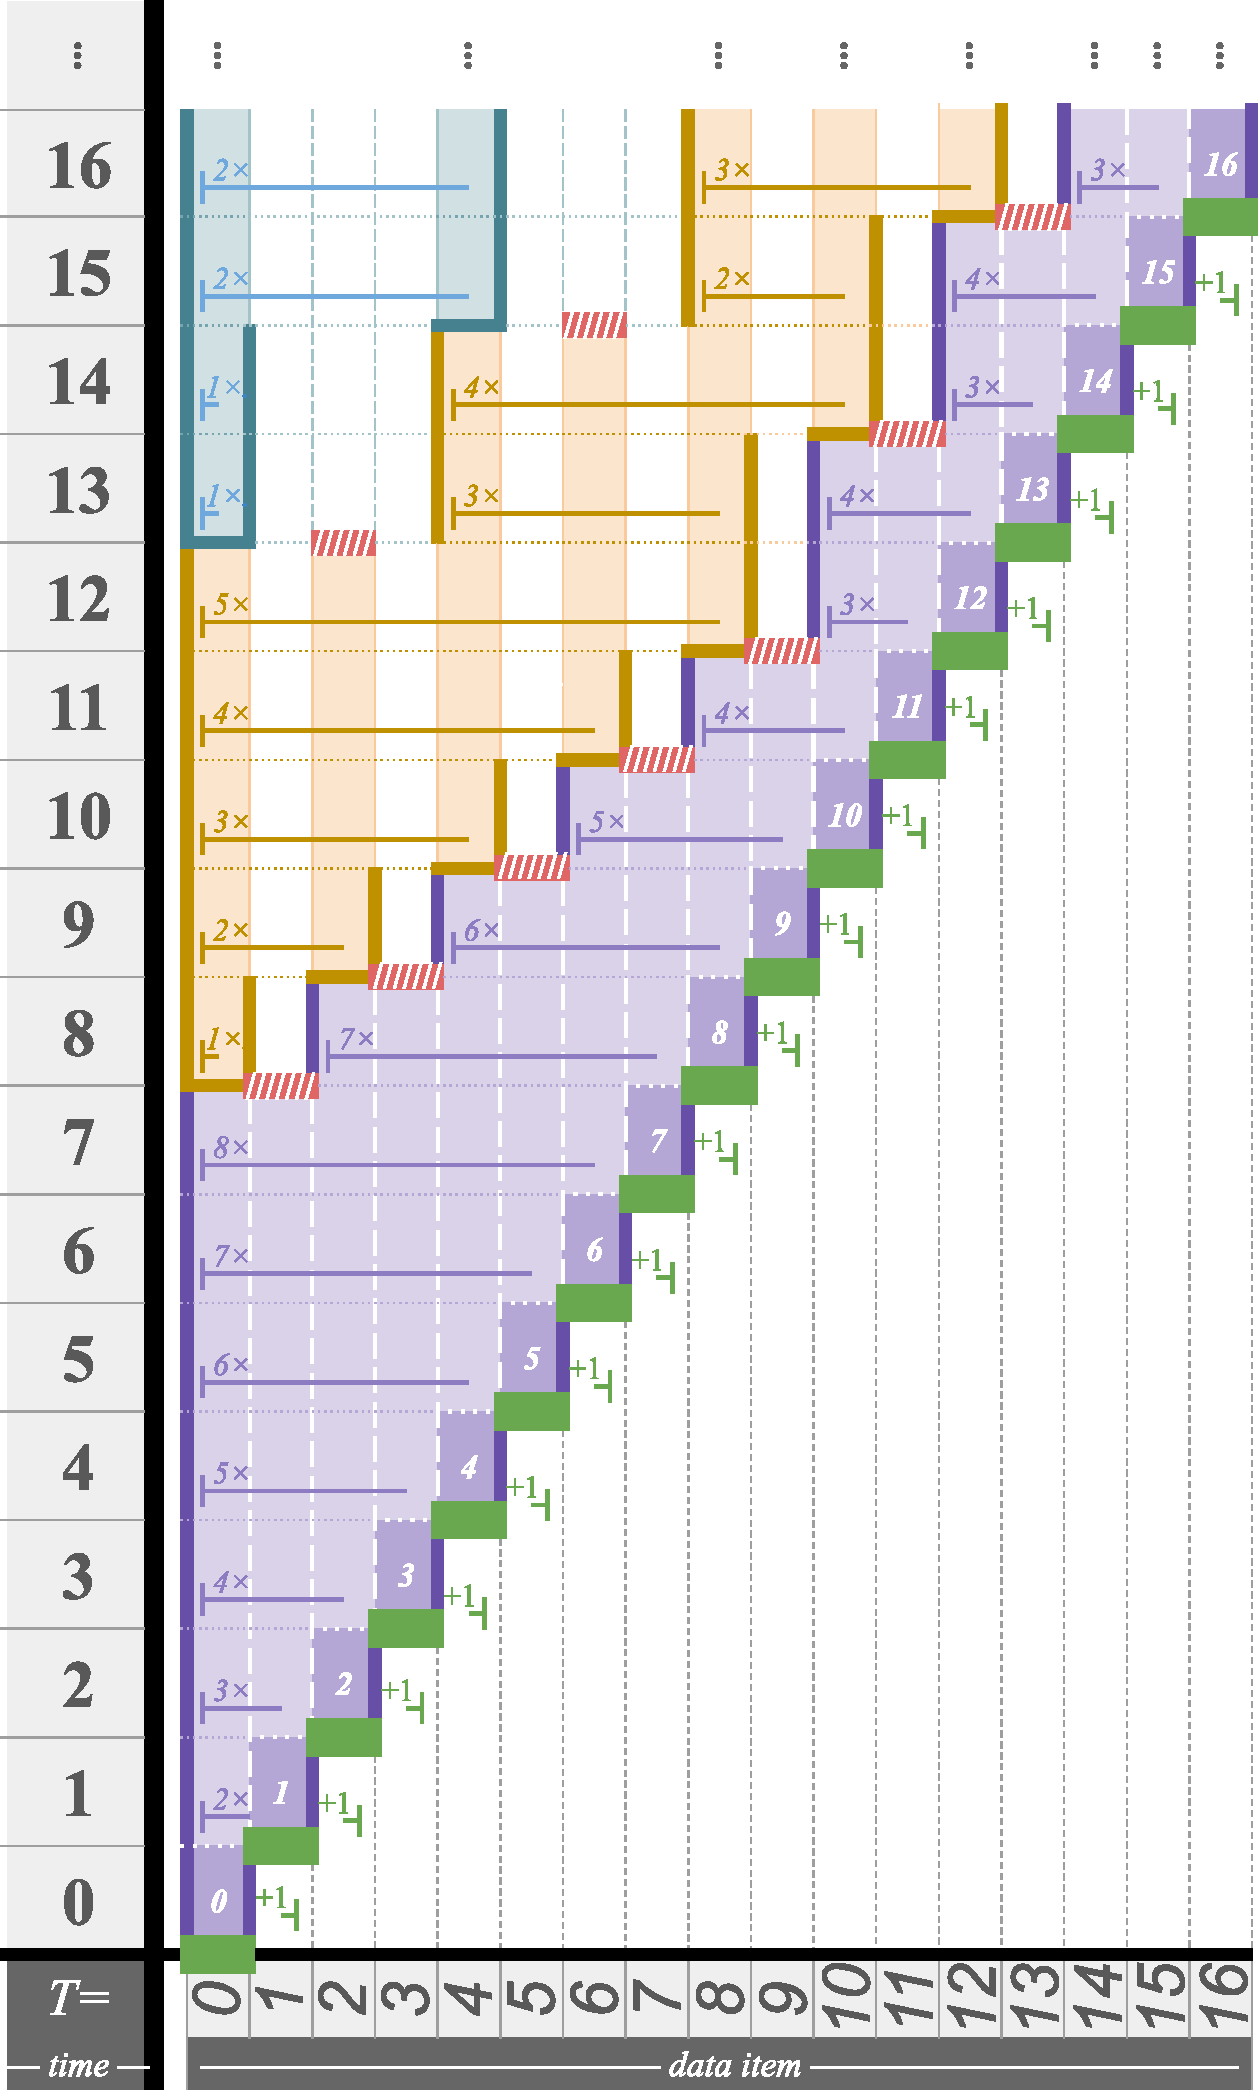
\includegraphics[height=4in,trim={2.5cm 0 0 0},clip]{img/surface-control-tall-zhao-full}
\centering
\caption{saturating bucket algorithm (Listing \ref{alg:zhao-tilted-full})}
\label{fig:surface-control-tilted:saturating-bucket}
\end{subfigure}

% graphics from https://docs.google.com/presentation/d/1wUBwtvcawkSLw5TL-7d7jybp6TXB4Pi5s6FyXDcHB8M

\caption{%
\textbf{Comparator tilted stream curation algorithms.}
\footnotesize
Example buffer state sequences, from top to bottom.
Stored data items shown as stream arrival index (hexidecimal notation).
For panels \cref{fig:surface-control:zhao-steady,fig:surface-control:zhao-tilted-ext}, buckets indicated by braced groupings.
}
\label{fig:surface-control-tilted}

\end{figure*}
